\documentclass[14pt]{extbook}
\usepackage{multicol, enumerate, enumitem, hyperref, color, soul, setspace, parskip, fancyhdr} %General Packages
\usepackage{amssymb, amsthm, amsmath, latexsym, units, mathtools} %Math Packages
\everymath{\displaystyle} %All math in Display Style
% Packages with additional options
\usepackage[headsep=0.5cm,headheight=12pt, left=1 in,right= 1 in,top= 1 in,bottom= 1 in]{geometry}
\usepackage[usenames,dvipsnames]{xcolor}
\usepackage{dashrule}  % Package to use the command below to create lines between items
\newcommand{\litem}[1]{\item#1\hspace*{-1cm}\rule{\textwidth}{0.4pt}}
\pagestyle{fancy}
\lhead{Progress Quiz 8}
\chead{}
\rhead{Version C}
\lfoot{5493-4176}
\cfoot{}
\rfoot{Summer C 2021}
\begin{document}

\begin{enumerate}
\litem{
Determine the horizontal and/or oblique asymptotes in the rational function below.\[ f(x) = \frac{6x^{3} +5 x^{2} -13 x -12}{2x^{2} +x -6} \]\begin{enumerate}[label=\Alph*.]
\item \( \text{Horizontal Asymptote at } y = -2.0 \)
\item \( \text{Horizontal Asymptote of } y = 3.0 \text{ and Oblique Asymptote of } y = 3x + 1 \)
\item \( \text{Horizontal Asymptote of } y = -2.0 \text{ and Oblique Asymptote of } y = 3x + 1 \)
\item \( \text{Horizontal Asymptote of } y = 3.0  \)
\item \( \text{Oblique Asymptote of } y = 3x + 1. \)

\end{enumerate} }
\litem{
Determine the vertical asymptotes and holes in the rational function below.\[ f(x) = \frac{4x^{3} -4 x^{2} -33 x + 45}{8x^{2} -14 x -15} \]\begin{enumerate}[label=\Alph*.]
\item \( \text{Vertical Asymptote of } x = 0.5 \text{ and hole at } x = 2.5 \)
\item \( \text{Vertical Asymptotes of } x = -0.75 \text{ and } x = 2.5 \text{ with no holes.} \)
\item \( \text{Vertical Asymptote of } x = -0.75 \text{ and hole at } x = 2.5 \)
\item \( \text{Vertical Asymptotes of } x = -0.75 \text{ and } x = 1.5 \text{ with a hole at } x = 2.5 \)
\item \( \text{Holes at } x = -0.75 \text{ and } x = 2.5 \text{ with no vertical asymptotes.} \)

\end{enumerate} }
\litem{
Determine the horizontal and/or oblique asymptotes in the rational function below.\[ f(x) = \frac{4x^{2} -11 x + 6}{20x^{3} -43 x^{2} +29 x -6} \]\begin{enumerate}[label=\Alph*.]
\item \( \text{Horizontal Asymptote of } y = 0 \)
\item \( \text{Horizontal Asymptote of } y = 0.200  \)
\item \( \text{Horizontal Asymptote at } y = 2.000 \)
\item \( \text{Oblique Asymptote of } y = 5x + 3. \)
\item \( \text{Horizontal Asymptote of } y = 0.200 \text{ and Oblique Asymptote of } y = 5x + 3 \)

\end{enumerate} }
\litem{
Which of the following functions \textit{could} be the graph below?
\begin{center}
    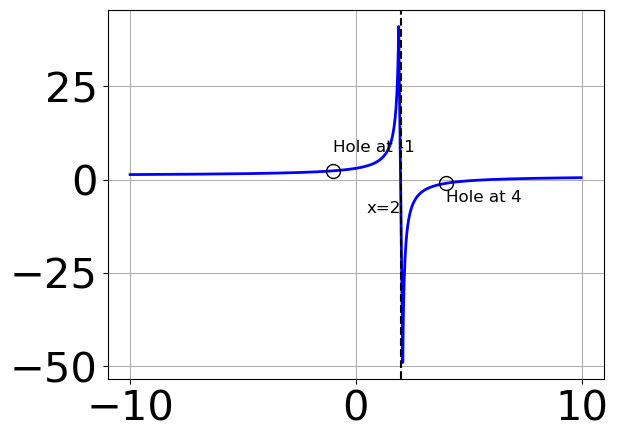
\includegraphics[width=0.5\textwidth]{../Figures/identifyGraphOfRationalFunctionC.png}
\end{center}
\begin{enumerate}[label=\Alph*.]
\item \( f(x)=\frac{x^{3} +3.0 x^{2} -34.0 x -120.0}{x^{3} -5.0 x^{2} +2.0 x + 8.0} \)
\item \( f(x)=\frac{x^{3} +12.0 x^{2} +41.0 x + 30.0}{x^{3} +5.0 x^{2} +2.0 x -8.0} \)
\item \( f(x)=\frac{x^{3} -9.0 x^{2} +14.0 x + 24.0}{x^{3} -5.0 x^{2} +2.0 x + 8.0} \)
\item \( f(x)=\frac{x^{3} +9.0 x^{2} +14.0 x -24.0}{x^{3} +5.0 x^{2} +2.0 x -8.0} \)
\item \( \text{None of the above are possible equations for the graph.} \)

\end{enumerate} }
\litem{
Determine the vertical asymptotes and holes in the rational function below.\[ f(x) = \frac{9x^{3} +27 x^{2} -4 x -12}{6x^{2} -5 x -6} \]\begin{enumerate}[label=\Alph*.]
\item \( \text{Vertical Asymptotes of } x = 1.5 \text{ and } x = -0.667 \text{ with no holes.} \)
\item \( \text{Holes at } x = 1.5 \text{ and } x = -0.667 \text{ with no vertical asymptotes.} \)
\item \( \text{Vertical Asymptote of } x = 1.5 \text{ and hole at } x = -0.667 \)
\item \( \text{Vertical Asymptote of } x = 1.5 \text{ and hole at } x = -0.667 \)
\item \( \text{Vertical Asymptotes of } x = 1.5 \text{ and } x = 0.667 \text{ with a hole at } x = -0.667 \)

\end{enumerate} }
\litem{
Determine the horizontal and/or oblique asymptotes in the rational function below.\[ f(x) = \frac{6x^{3} -25 x^{2} +x + 60}{3x^{2} -2 x -8} \]\begin{enumerate}[label=\Alph*.]
\item \( \text{Horizontal Asymptote at } y = 2.0 \)
\item \( \text{Horizontal Asymptote of } y = 2.0 \text{ and Oblique Asymptote of } y = 2x -7 \)
\item \( \text{Horizontal Asymptote of } y = 2.0 \text{ and Oblique Asymptote of } y = 2x -7 \)
\item \( \text{Horizontal Asymptote of } y = 2.0  \)
\item \( \text{Oblique Asymptote of } y = 2x -7. \)

\end{enumerate} }
\litem{
Determine the horizontal and/or oblique asymptotes in the rational function below.\[ f(x) = \frac{24x^{3} -38 x^{2} -45 x + 50}{-30x^{3} +20 x^{2} +35 x -50} \]\begin{enumerate}[label=\Alph*.]
\item \( \text{None of the above} \)
\item \( \text{Horizontal Asymptote of } y = 0  \)
\item \( \text{Vertical Asymptote of } y = -1.000  \)
\item \( \text{Vertical Asymptote of } y = 2  \)
\item \( \text{Horizontal Asymptote of } y = -0.800  \)

\end{enumerate} }
\litem{
Which of the following functions \textit{could} be the graph below?
\begin{center}
    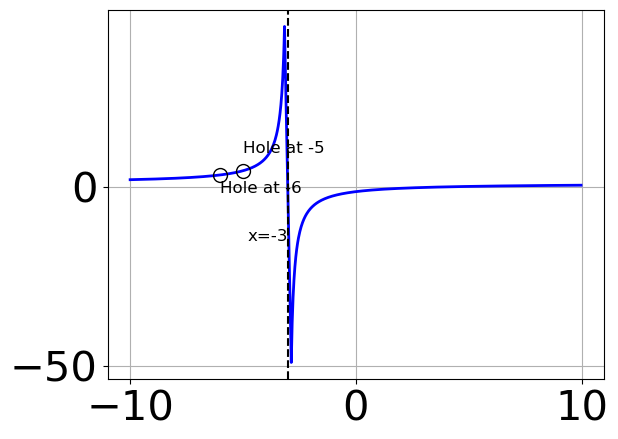
\includegraphics[width=0.5\textwidth]{../Figures/identifyGraphOfRationalFunctionCopyC.png}
\end{center}
\begin{enumerate}[label=\Alph*.]
\item \( f(x)=\frac{x^{3} +7.0 x^{2} -14.0 x -120.0}{x^{3} +14.0 x^{2} +63.0 x + 90.0} \)
\item \( f(x)=\frac{x^{3} +8.0 x^{2} +19.0 x + 12.0}{x^{3} -14.0 x^{2} +63.0 x -90.0} \)
\item \( f(x)=\frac{x^{3} -7.0 x^{2} -14.0 x + 120.0}{x^{3} -14.0 x^{2} +63.0 x -90.0} \)
\item \( f(x)=\frac{x^{3} -8.0 x^{2} +11.0 x + 20.0}{x^{3} +14.0 x^{2} +63.0 x + 90.0} \)
\item \( \text{None of the above are possible equations for the graph.} \)

\end{enumerate} }
\litem{
Determine the vertical asymptotes and holes in the rational function below.\[ f(x) = \frac{6x^{3} -31 x^{2} +53 x -30}{6x^{2} +5 x -25} \]\begin{enumerate}[label=\Alph*.]
\item \( \text{Vertical Asymptotes of } x = -2.5 \text{ and } x = 1.5 \text{ with a hole at } x = 1.667 \)
\item \( \text{Vertical Asymptote of } x = 1.0 \text{ and hole at } x = 1.667 \)
\item \( \text{Vertical Asymptotes of } x = -2.5 \text{ and } x = 1.667 \text{ with no holes.} \)
\item \( \text{Vertical Asymptote of } x = -2.5 \text{ and hole at } x = 1.667 \)
\item \( \text{Holes at } x = -2.5 \text{ and } x = 1.667 \text{ with no vertical asymptotes.} \)

\end{enumerate} }
\litem{
Determine the vertical asymptotes and holes in the rational function below.\[ f(x) = \frac{9x^{3} +15 x^{2} -74 x + 40}{6x^{2} -13 x + 6} \]\begin{enumerate}[label=\Alph*.]
\item \( \text{Vertical Asymptotes of } x = 1.5 \text{ and } x = 0.667 \text{ with no holes.} \)
\item \( \text{Vertical Asymptote of } x = 1.5 \text{ and hole at } x = 0.667 \)
\item \( \text{Vertical Asymptote of } x = 1.5 \text{ and hole at } x = 0.667 \)
\item \( \text{Holes at } x = 1.5 \text{ and } x = 0.667 \text{ with no vertical asymptotes.} \)
\item \( \text{Vertical Asymptotes of } x = 1.5 \text{ and } x = 1.667 \text{ with a hole at } x = 0.667 \)

\end{enumerate} }
\end{enumerate}

\end{document}